\documentclass[xcolor=dvipsnames,hyperref={breaklinks=true},mathserif,professionalfont,dvipdfmx,12pt]{beamer}
\usepackage[ipaex]{pxchfon}
\usepackage{amsmath,amssymb}
\usepackage{amsthm}
\usepackage{ascmac}

\usepackage[utf8]{inputenc}
\usepackage{bm}
\usepackage{here}
\usepackage{enumerate}
\usepackage{bxdpx-beamer} %dvipdfmc対応
\usepackage{pxjahyper} %しおりの和文対応
\usepackage{minijs} %jsarticleのミニ版
\usepackage{otf}
\usepackage{helvet}
\usepackage{breqn}
\usepackage{color}
\usepackage{xcolor}
\usepackage{graphicx}

\usepackage[style=chem-angew,backend=bibtex]{biblatex}
\AtEveryCitekey{\iffootnote{\tiny}{}}
\usepackage{filecontents}
\addbibresource{Reference.bib}


%hyperlink等
\usepackage{hyperref}
\usepackage{pxjahyper}

\renewcommand{\kanjifamilydefault}{\gtdefault}
%TikZ
\usepackage{tikz}
\usetikzlibrary{positioning}
\usetikzlibrary{arrows.meta}
\usetikzlibrary{bending}
\usetikzlibrary{shapes.geometric}
\usetikzlibrary {shapes.misc}

\usepackage[T1]{fontenc}
\usepackage{lmodern}
\usepackage{gnuplot-lua-tikz}
\usepackage{gnuplottex}

\usepackage[absolute,overlay]{textpos}
% \usepackage[colorgrid,gridunit=pt,texcoord]{eso-pic}%グリッド表示


\renewcommand{\figurename}{図}
\renewcommand{\tablename}{表}


\setbeamertemplate{caption}[numbered]

\title{Hidden Fluid Mechanics: A Navier-Stokes Informed Deep Learning Framework for Assimilating Flow Visualization Data}
\author{YokoPhys-h}
\date{\today}
\institute{hoge大学大学院}
\titlegraphic{
\includegraphics[scale=0.3]{icon_YokoPhys.png}}




% \usetheme{Madrid}
\usetheme{Montpellier}
% \usetheme{AnnArbor}
%\usetheme{Copenhagen}
% \usecolortheme[RGB={0, 126, 15}]{structure}

% \usetheme{Rochester}

\usecolortheme[named=Blue]{structure} % 色指定
\usefonttheme{professionalfonts}

\setbeamertemplate{blocks}[rounded][shadow=true]
%itemizeの記号設定
\setbeamertemplate{itemize item}[default] 
\setbeamertemplate{itemize subitem}[triangle]
\setbeamertemplate{itemize subsubitem}[circle]

% \setbeamertemplate{navigation symbols}{}%ナビゲーションシンボル消去
\setbeamertemplate{footline}[page number] %ページ番号
%\setbeamertemplate{navigation symbols}[horizontal]

\makeatletter
\def\pgfutil@insertatbegincurrentpagefrombox#1{%
  \edef\pgf@temp{\the\wd\pgfutil@abb}%
  \global\setbox\pgfutil@abb\hbox{%
    \unhbox\pgfutil@abb%
    \hskip\dimexpr2in-2\hoffset-\pgf@temp\relax% changed
    #1%
    \hskip\dimexpr-2in-2\hoffset\relax% new
  }%
}
\makeatother


\begin{document}

\begin{frame}[plain]
  \titlepage
\end{frame}
\begin{frame}
  \frametitle{Contents}
  \tableofcontents
\end{frame}


\section{Hidden Fluid Mechanics (HFM)}
\begin{frame}
  \frametitle{Hidden Fluid Mechanics (HFM)}
  \vspace{10pt}
  \structure{流れのダイナミクスを調べる}
  \begin{itemize}
    \item Navier-Stokes方程式の直接的数値計算\\
    \footnotesize$\rightarrow$並列計算, Neural Networksによる微分方程式の求解, etc.\normalsize 
    \item 実験観測的手法\\
    \footnotesize$\rightarrow$ データ記録装置, センサー技術\normalsize
  \end{itemize}
  \structure{データ同化}\\
  \small 数値モデルの再現性を高める.\normalsize
  \begin{itemize}
    \item 数値計算結果+実験観測データ $\rightarrow$パラメータ決定, モデルの再構築
  \end{itemize}
\end{frame}

\begin{frame}
  \structure{流れのダイナミクスの潜在物理量}\\
  \small 流れの表面だけでなく, 内部の情報を知りたい. (例: 流速, 圧力, etc.)\normalsize
  \begin{itemize}
    \item 実験観測的手法\\
    \footnotesize レーザーイメージング, 粒子画像流速測定法, Computer Tomography (CT), etc.\normalsize
    \item 理論的手法\\
    \footnotesize $\rightarrow$ spectral/hp-element solver : NekTar\normalsize
  \end{itemize}
  すごく大変.
\end{frame}

\begin{frame}
  \structure{Physics Informed Neural Networks (PINNs)}\footfullcite{RAISSI2019686}\\
  \small Neural Networkの損失関数に物理的制約を取り込むことで, 学習データを必要とせず, 関数を出力する.\normalsize
  \begin{figure}[H]
    \centering
      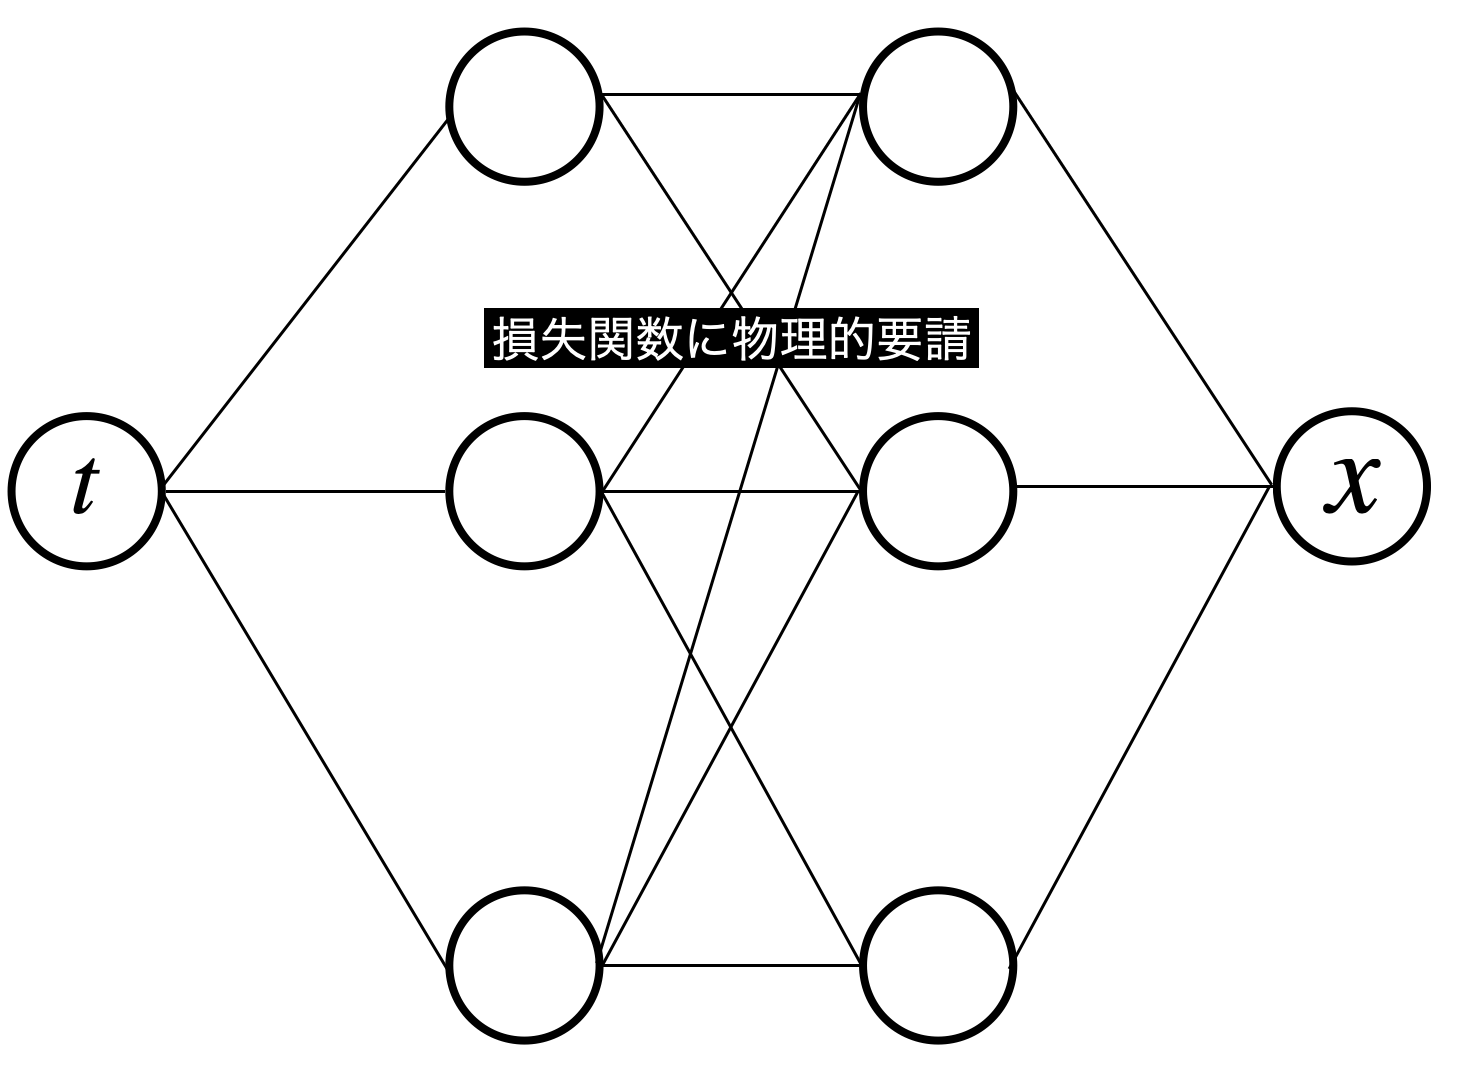
\includegraphics[width=0.5\linewidth]{figure/fig10.png}
  \end{figure}
\end{frame}

\begin{frame}
  \structure{Physics Informed Neural Networks (PINNs)}\footfullcite{RAISSI2019686}\\
  \small Neural Networkの損失関数に物理的制約を取り込むことで, 学習データを必要とせず, 関数を出力する.\normalsize
  \footnotesize
  \begin{itemize}
    \item 実験観測データと理論(物理的制約)を組み合わせて流体の内部情報を拾えないか?
  \end{itemize}\normalsize
  \begin{tikzpicture}
    \tikzset{Process/.style={rectangle,  draw,  text centered, text width=5cm, minimum height=1cm}};
    \node[Process] (a) {\scriptsize 実験観測データ$\tiny\{t^n,x^n,y^n,z^n, c^n\}_{n=1}^{N}\normalsize$\\+\\理論(物理的要請)\\
    $\rho\left(\partial_{t} c+\boldsymbol{u} \cdot \nabla c\right)=\kappa \nabla^{2} c$\\
    $ \tiny\left\{\begin{array}{l}
      \rho\left(\partial_{t} \bm{u}+(\bm{u} \cdot \nabla) \bm{u}\right)=-\nabla p+\mu \Delta \bm{u}+\rho \bm{f} \\
      \operatorname{ divu }=0
      \end{array}\right.$\normalsize\normalsize};
    \node[Process][right=1.0cm of a] (b) {\scriptsize 関数出力\\
    $u(t, x, y, z), v(t, x, y, z)$,\\ $w(t, x, y, z) ,p(t, x, y, z)$\normalsize};
    \draw[->] (a) -- (b);
  \end{tikzpicture}
  \alert{$\rightarrow$ Hidden Fluid Mechanics (HFM)}\footfullcite{raissi_HiddenFluidMechanics_2018}
\end{frame}

\subsection{passive scalerの輸送現象}
\begin{frame}
  \frametitle{Hidden Fluid Mechanics (HFM)}
  \structure{passive scalerの輸送現象} \small (例: spreading smoke, dye advected)\normalsize\\
  \scriptsize 流体運動そのものに力学的効果を与えない流れにおける拡散場の輸送 \normalsize\\
  \footnotesize \structure{輸送拡散方程式}\normalsize
  \begin{align*}
    \rho\left(\partial_t c+\bm{u}\cdot \nabla c\right)=\kappa\nabla^2c
  \end{align*}
  \footnotesize$\left(c: \text{scaler field}, \bm{u}: \text{velocity}, \kappa: \text{moleculer diffusinity}, \rho: \text{density}\right)$\normalsize\\
  \footnotesize \structure{Navier-Stokes方程式} \normalsize
  \footnotesize
  \begin{align*}
    \begin{aligned}
        &\rho\left(\partial_{t} \bm{u}+(\bm{u} \cdot \nabla) \bm{u}\right)=-\nabla p+\mathrm{Re}^{-1} \Delta \bm{u}s\\
        &\operatorname{div}\bm{u}=0
      \end{aligned}
  \end{align*}
  \footnotesize$\left(p: \text{pressuer}, \mathrm{Re}: \text{Reynolds number}\right)$\normalsize
\end{frame}

\subsection{計算準備}
\begin{frame}
  \frametitle{計算準備}
 \structure{実験観測データ}
 \begin{align*}
  \{t^n,x^n,y^n,z^n, c^n\}_{n=1}^{N}
 \end{align*}
  \structure{物理的要請}\\
    \small 輸送方程式:\normalsize
    \begin{align*}
      c_{t}+u c_{x}+v c_{y}+w c_{z}=\operatorname{Pec}^{-1}\left(c_{x x}+c_{y y}+c_{z z}\right)
    \end{align*}
    \small Navier-Stokes方程式:\normalsize
    \footnotesize
    \begin{align*}
      \begin{aligned}
      &u_{t}+u u_{x}+v u_{y}+w u_{z}=-p_{x}+\operatorname{Re}^{-1}\left(u_{x x}+u_{y y}+u_{z z}\right) \\
      &v_{t}+u v_{x}+v v_{y}+w v_{z}=-p_{y}+\operatorname{Re}^{-1}\left(v_{x x}+v_{y y}+v_{z z}\right) \\
      &w_{t}+u w_{x}+v w_{y}+w w_{z}=-p_{z}+\operatorname{Re}^{-1}\left(w_{x x}+w_{y y}+w_{z z}\right) \\
      &u_{x}+v_{y}+w_{z}=0
    \end{aligned}
    \end{align*}
    \normalsize
    \small \structure{精度向上}\normalsize \footnotesize$d_{t}+u d_{x}+v d_{y}+w d_{z}=\operatorname{Pec}^{-1}\left(d_{x x}+d_{y y}+d_{z z}\right),\quad (d:=1-c)$\normalsize
\end{frame}

\subsection{計算}
\begin{frame}
  \frametitle{計算}
  \structure{Neural Network} $\{t^n,x^n,y^n,z^n, c^n\}_{n=1}^{N}\longrightarrow(c,d,u,v,w,p)$
  \begin{figure}[H]
    \centering
      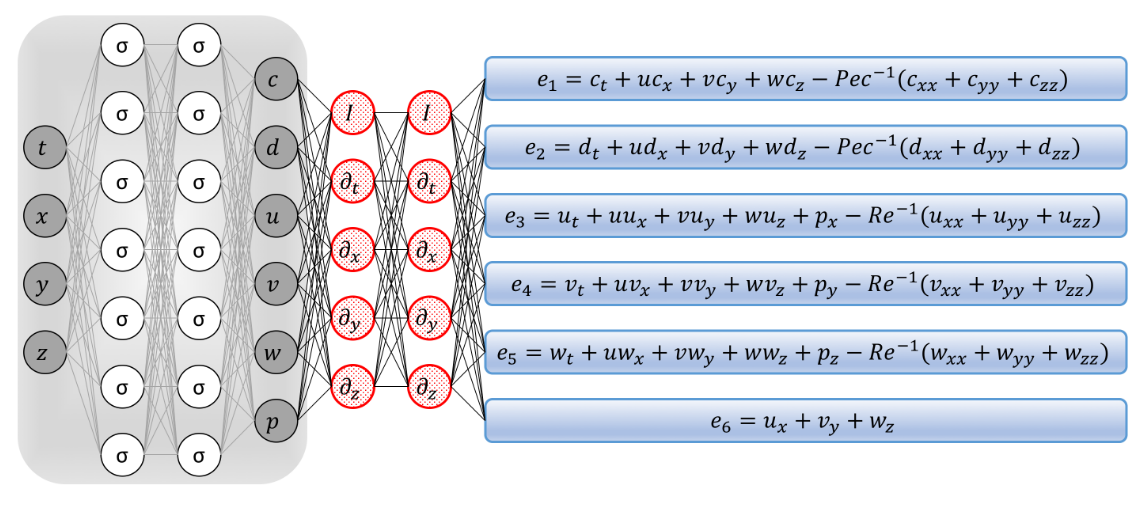
\includegraphics[width=0.8\linewidth]{figure/fig1.png}
  \end{figure}
  \vspace{-11pt}
  \structure{損失関数} 
  \footnotesize
  \begin{flalign*}
    &\begin{aligned}
      S S E &=\sum_{n=1}^{N}\left|c\left(t^{n}, x^{n}, y^{n}, z^{n}\right)-c^{n}\right|^{2}+\sum_{n=1}^{N}\left|d\left(t^{n}, x^{n}, y^{n}, z^{n}\right)-d^{n}\right|^{2}\\&+\sum_{i=1}^{6} \sum_{n=1}^{N}\left|e_{i}\left(t^{n}, x^{n}, y^{n}, z^{n}\right)\right|^{2}
      \end{aligned}&
  \end{flalign*}\normalsize
\end{frame}

\subsection{計算結果}
\begin{frame}
  \frametitle{計算結果}
  \structure{学習データ}\\
  円柱を通過する2次元流れ
  \begin{figure}[H]
    \centering
      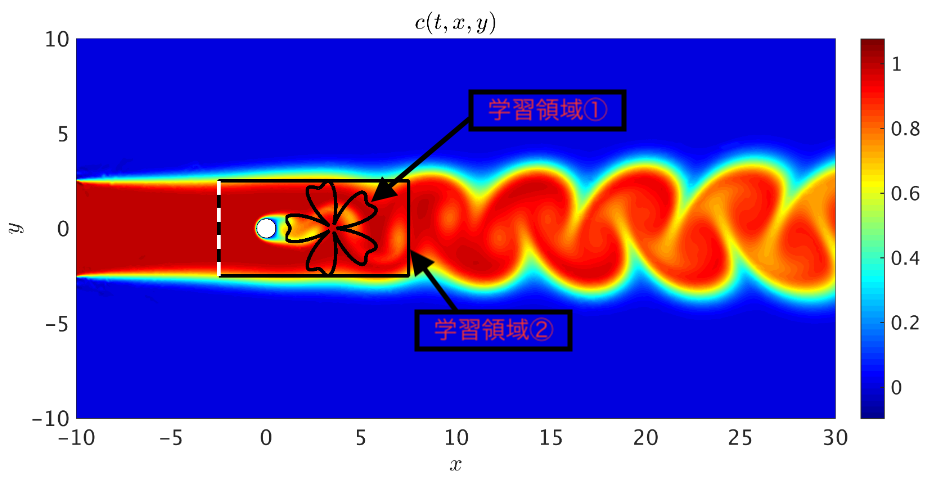
\includegraphics[width=1\linewidth]{figure/fig2.png}
  \end{figure}
\end{frame}

\begin{frame}[t]
  \structure{結果}
  \begin{figure}[H]
    \centering
      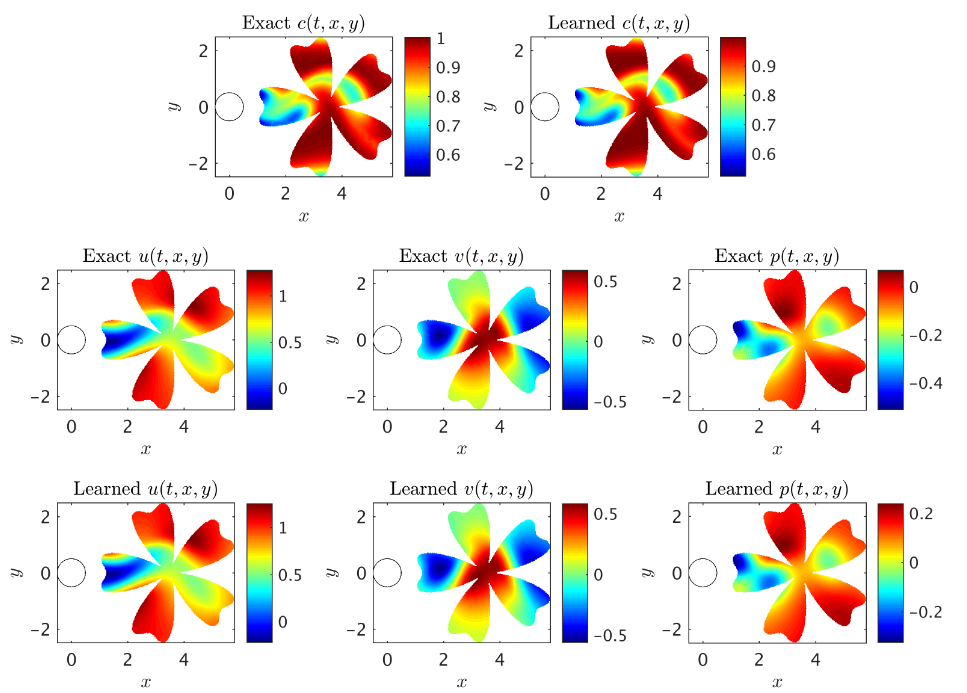
\includegraphics[width=0.9\linewidth]{figure/fig3.png}
  \end{figure}
  \begin{textblock*}{0.4\linewidth}(250pt, 70pt)
    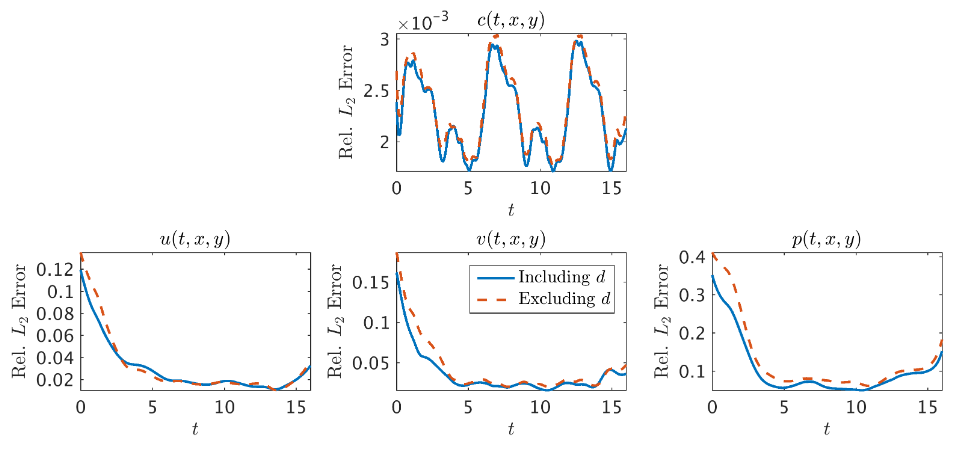
\includegraphics[width=\linewidth]{figure/fig4.png}
    \end{textblock*}
\end{frame}
\begin{frame}[t]
  \begin{figure}[H]
    \centering
      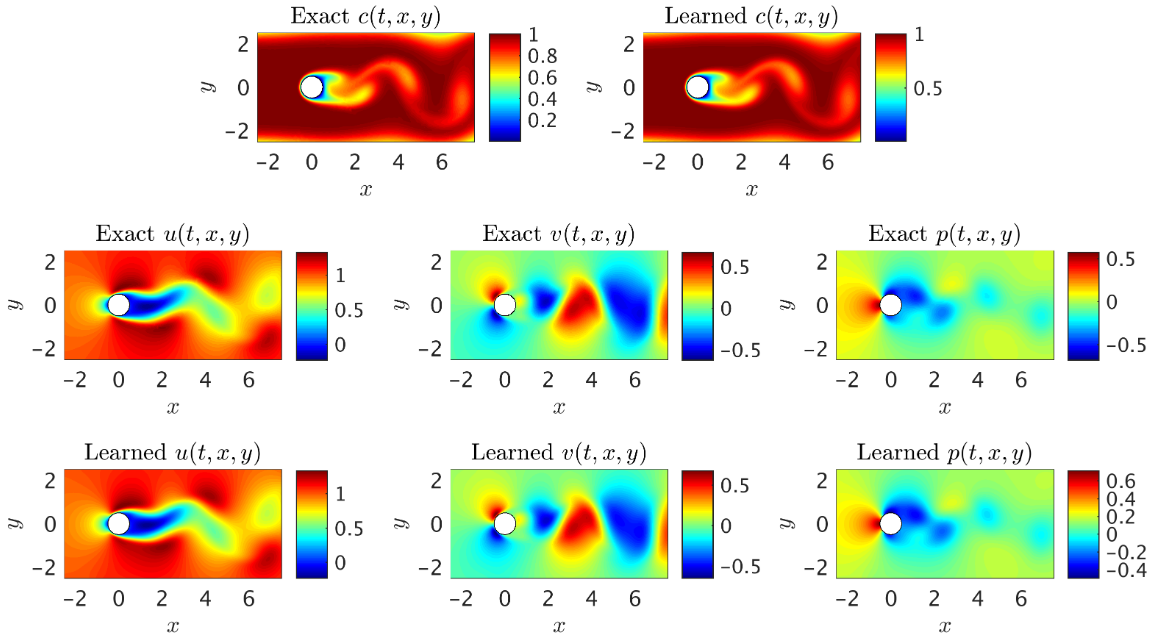
\includegraphics[width=0.9\linewidth]{figure/fig5.png}
  \end{figure}
  \begin{textblock*}{0.5\linewidth}(20pt, 205pt)
    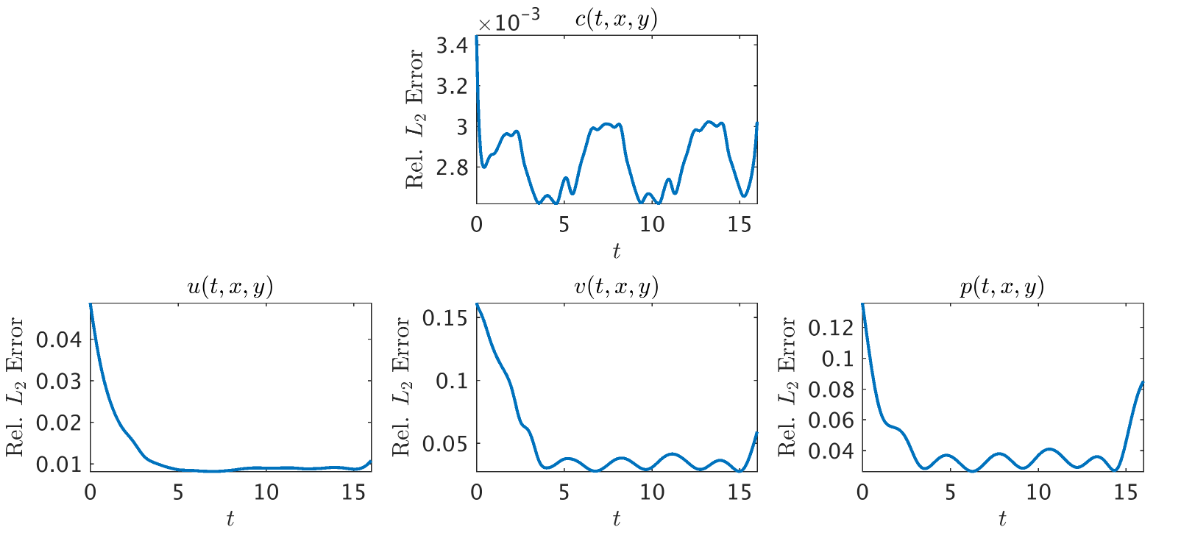
\includegraphics[width=\linewidth]{figure/fig6.png}
    \end{textblock*}
\end{frame}

\subsection{利点とまとめ}
\begin{frame}
  \frametitle{利点とまとめ}
  \setbeamertemplate{itemize item}[ball]
  \begin{itemize}
    \item 使用したのは実験観測データと基礎方程式のみ
    \begin{itemize}
      \item 拘束条件がわからない状況でも, 流体内部の速度, 圧力を推定できる.
      \item 境界壁に囲まれている内部の流れの速度や圧力なども正しく形状を定義せずとも算出できる.
    \end{itemize}
    \item 関数が出力される
    \begin{itemize}
      \item パラメータを逆に決めることもできる.
      \begin{figure}[H]
        \centering
          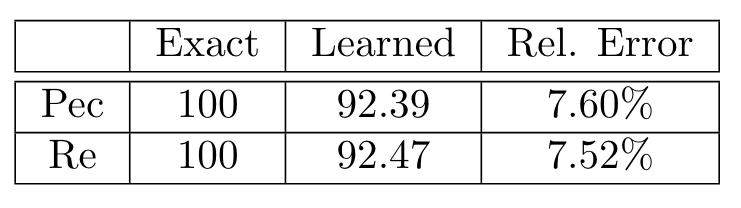
\includegraphics[width=0.5\linewidth]{figure/fig7.png}
      \end{figure}
    \end{itemize}
  \end{itemize}
  \structure{HFMを使うことで詳しく初期条件や境界条件を知らずとも物理的制約(保存即, 運動方程式)のみで現象の内部の情報を拾うことができるようになる.}\\
  \footnotesize$\rightarrow$ 生体内内部情報(血液流速, 応力, etc.), 連続体内部情報(浮力, 応力, etc.)への有用可能性.\normalsize
\end{frame}



% 参考文献
\begin{frame}[allowframebreaks]{参考文献}
  \printbibliography
\end{frame}

\section{Appendix}
\subsection{3次元データへの適用}
\begin{frame}[t]
\structure{学習データ}
  \begin{figure}[H]
    \centering
      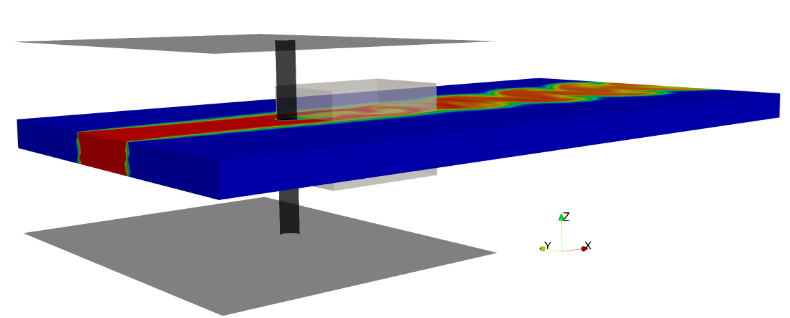
\includegraphics[width=1\linewidth]{figure/fig8.png}
  \end{figure}
\end{frame}

\begin{frame}
  \structure{結果}
  \begin{figure}[H]
    \centering
      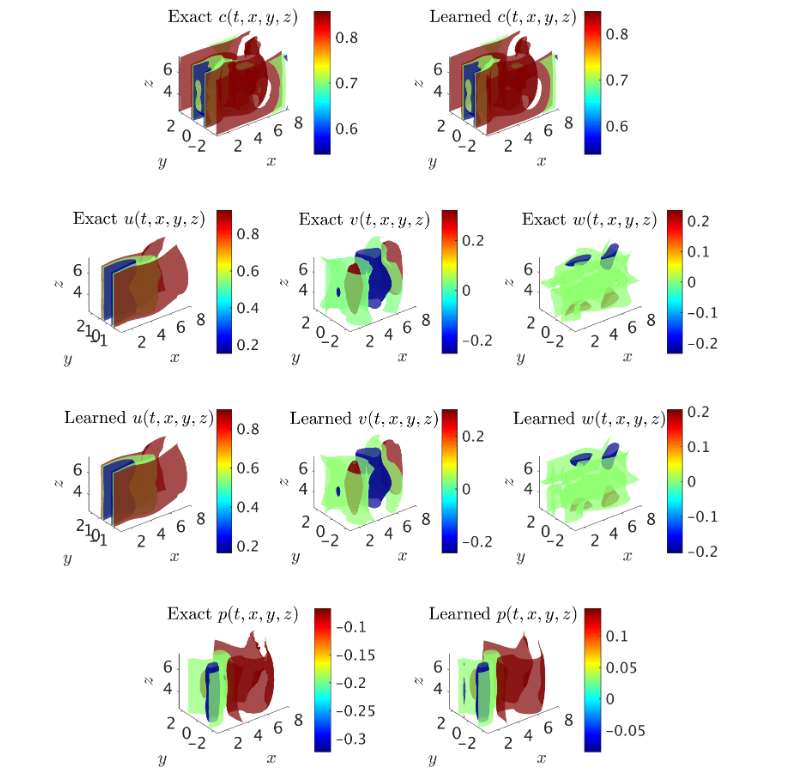
\includegraphics[width=0.7\linewidth]{figure/fig9.png}
  \end{figure}
\end{frame}



% \frame{\centering \Large Thank you for your attention !!}


\end{document}